\renewcommand{\theequation}{\theenumi}
\begin{enumerate}[label=\thesection.\arabic*.,ref=\thesection.\theenumi]
\numberwithin{equation}{enumi}

\begin{figure}[!ht]
\centering
\resizebox{\columnwidth}{!}{\begin{tikzpicture}[scale = 1.5,>=stealth,point/.style={draw,circle,fill=black, inner sep=0.5pt},]

\node (Q) at (0, 0)[point,label=below left:$Q$] {};
\node (R) at (6, 0)[point,label=below right:$R$] {};
\node (P) at (2.25, 3.307189138830738)[point,label=above right:$P$] {};
\node (S) at (8/3, 0)[point,label=below:$S$] {};
\node (G) at (4/3, 0)[label=below:$y$] {};

\draw (P) -- node[below=5pt]{}(Q) -- (R) -- (P) -- (S);

\tkzMarkAngle[fill=green!20, mark=|](Q,P,S)
\tkzMarkAngle[fill=green!20, mark=|](S,P,R)

\end{tikzpicture}}
\caption{Quadilateral by Latex-Tikz}
\label{fig:triangle1}	
\end{figure}

\item The figure obtained looks like Fig. \ref{fig:triangle1}.
$PR > PQ$, $\angle{QPS}=\angle{SPR}=x$

\item The design parameters used for construction are :
$$QR = p = 6$$
$$PR = q = 5$$
$$PQ = r = 4$$

\item Point $S$ can be found by Triangle angle bisector theorem.
$$QS/PQ = SR/PR$$
$$y/4 = (6-y)/5$$
$$5y = 24 - 4y$$
$$9y = 24$$
$$y = 8/3$$

\item Draw fig. \ref{fig:triangle2}.

\begin{figure}[!ht]
\centering
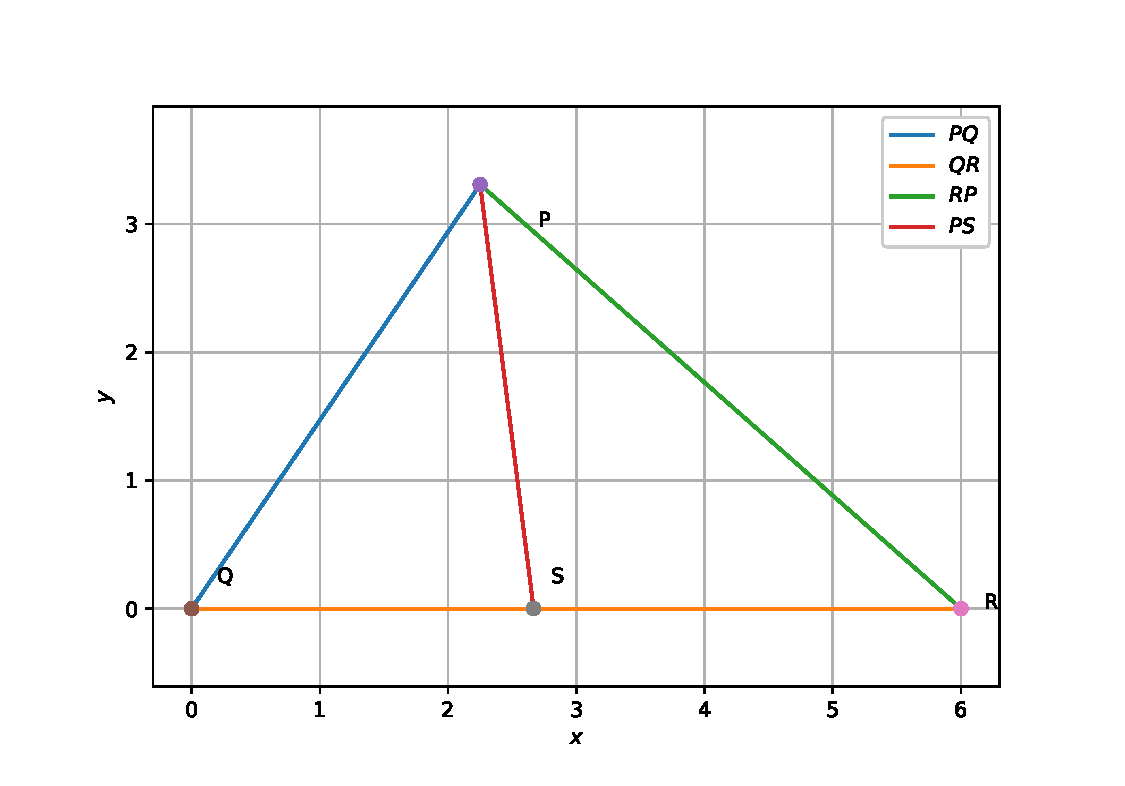
\includegraphics[width=\columnwidth]{./codes/tri.eps}
\caption{Triangle generated using python}
\label{fig:triangle2}
\end{figure} 

\solution The  following Python code generates Fig. \ref{fig:triangle2}

\begin{lstlisting}
codes/tri.py
\end{lstlisting}

and the equivalent latex-tikz code generating Fig. \ref{fig:triangle2} is 
\begin{lstlisting}
figs/triangle.tex
\end{lstlisting}
%
%The above latex code can be compiled as a standalone document as
%\begin{lstlisting}
%figs/quad_final.tex
%end{lstlisting}
\end{enumerate}
  

